\begin{figure}
	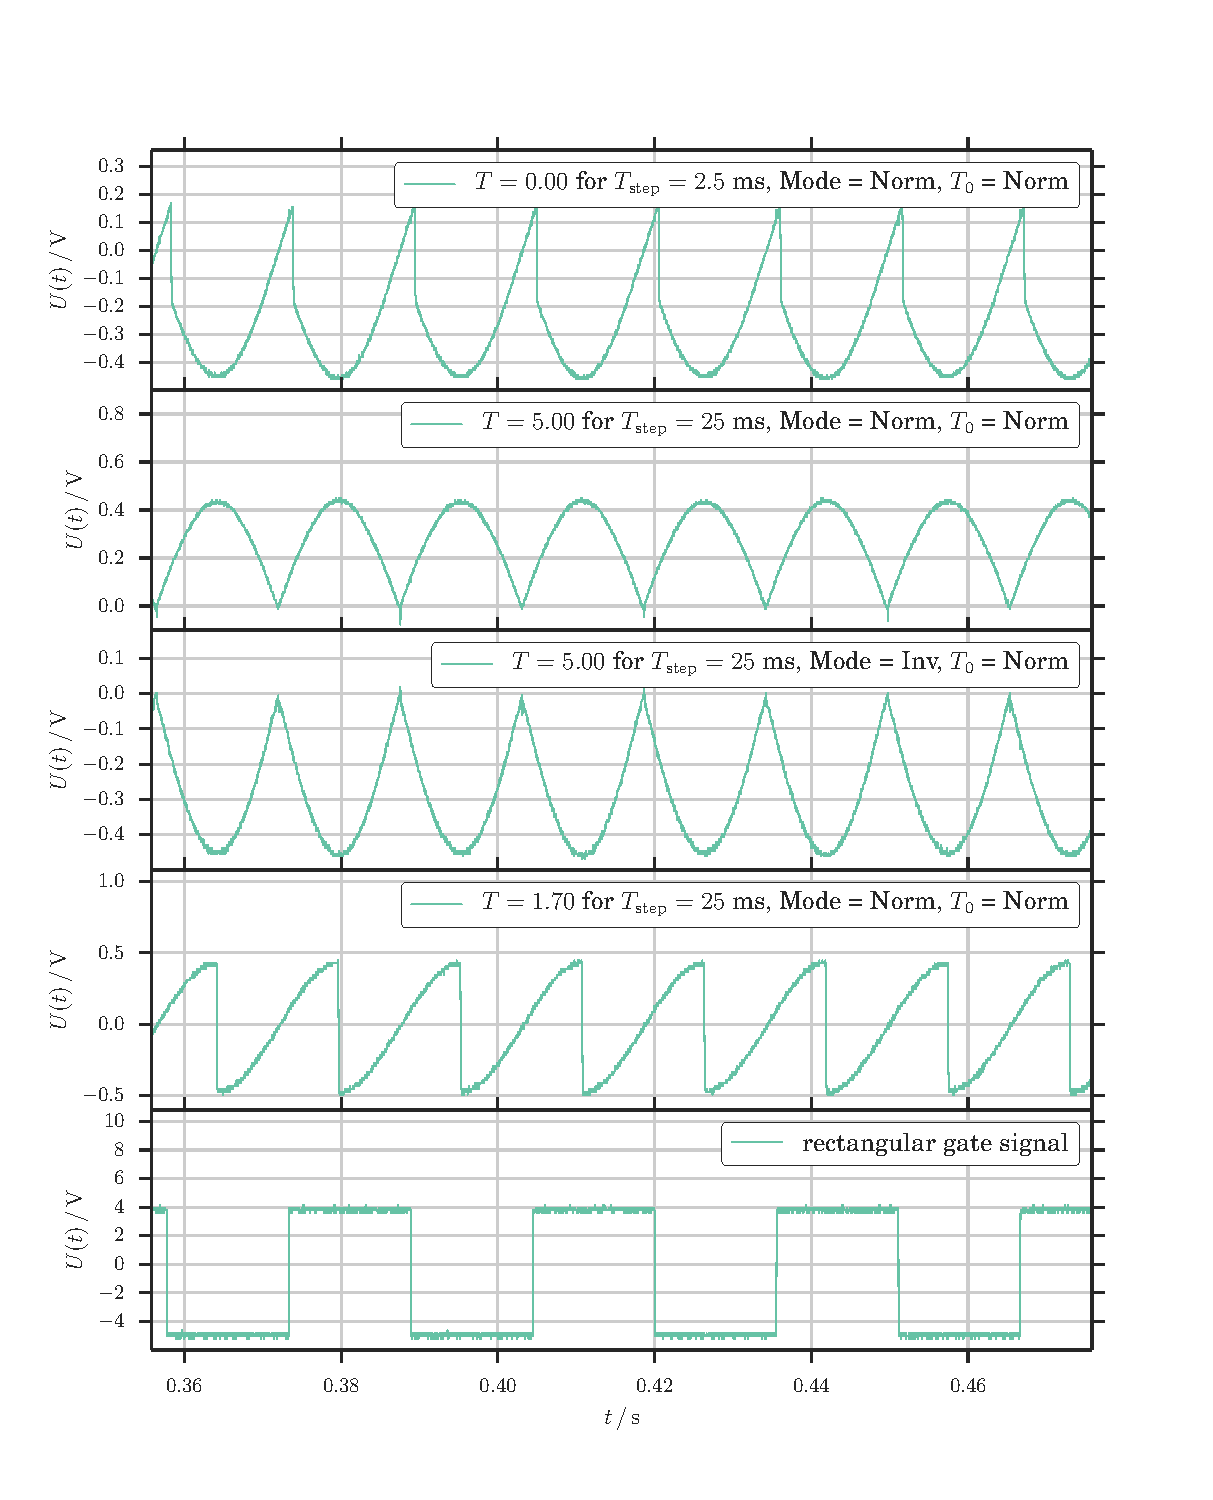
\includegraphics[width=\textwidth]{figures/phase.pdf}
	\caption{
		Lock-in phase calibration.
		$T$ indicates the value shown on the potentiometer 'Time Const', 
		the following three parameters correspond to the toggle switches located on the lock-in analyser.
		One can make the following observations: For $T = 0$, the phase difference $\Delta \phi$ is not zero;
		the inversion does not change the signal's form but only the sign; The phase differences corresponding 
		to the lower three signals are $\Delta \phi = 2\pi, \pi, \pi / 2$, respectively.
		The error on $T$ is given by $s_T = 0.03$.
		}
	\label{fig:phase}
\end{figure}

